\documentclass[12pt, a4paper, oneside]{article}
\usepackage[UTF8]{ctex}
\usepackage{amsmath, amsthm, amssymb, bm, framed, graphicx, subcaption, mathrsfs, physics}
\usepackage{xcolor}
\usepackage{tikz}
\usetikzlibrary{calc, arrows}
\usepackage{siunitx}
\usepackage[unicode]{hyperref}
\usepackage[capitalise]{cleveref}

\definecolor{shadecolor}{RGB}{241, 241, 255}

\sisetup{
  inter-unit-product = \ensuremath{{}\cdot{}},  % 单位间用点乘
  exponent-product  = \times,                  % 科学计数法用 × 而非 e
  group-separator   = {\,},                    % 千分位窄空格分隔
  separate-uncertainty                         % 不确定度用 ± 符号
}

\hypersetup{
  CJKbookmarks = true,
  bookmarksnumbered = true,
  pdfstartview = FitH,
  colorlinks = true,
  linkcolor = blue,
  anchorcolor = black,
  citecolor = green,
}

% 自定义公式引用格式
\crefname{equation}{Eq.}{Eq.}
\Crefname{equation}{Eq.}{Eq.}
\crefformat{equation}{Eq.(#2#1#3)}
\Crefformat{equation}{Eq.(#2#1#3)}

% 保持图和表格的默认引用格式
\renewcommand{\figurename}{Fig.}
\crefname{figure}{Fig.}{Figs.}
\renewcommand{\tablename}{Tab.}
\crefname{table}{Tab.}{Tabs.}

% % 定义 autoref 标签名
% \def\figureautorefname{Fig.}
% \def\tableautorefname{Tab.}
% \def\equationautorefname{Eq.}

\title{\textbf{MIT GR Course Problem Set 1}\\Solutions and Explanations}
\author{Peter Benjamin Zhu}
\date{}
\linespread{1.5}
\definecolor{shadecolor}{RGB}{241, 241, 255}
\newcounter{problemname}
\newenvironment{problem}{\begin{shaded}\stepcounter{problemname}\par\noindent\textbf{Problem\arabic{problemname}. }}{\end{shaded}\par}
\newenvironment{solution}{\par\noindent\textbf{Solution. }}{\par}
\newenvironment{note}{\par\noindent\textbf{Notes for Problem\arabic{problemname}. }}{\par}

\newcommand{\vc}[1]{\ensuremath{\overrightarrow{#1}}}
\renewcommand{\vb}[1]{\ensuremath{\mathbf{#1}}}
\newcommand{\p}{\partial}
\newcommand{\e}{\ensuremath{\mathrm{e}}}

% 定义 \pv 命令(支持偏导数)
\DeclareDocumentCommand{\pv}{omg}{%
    \ensuremath{%
    \IfNoValueTF{#3}
    {\frac{\partial \IfNoValueTF{#1}{}{^{#1}}}{\partial #2\IfNoValueTF{#1}{}{^{#1}}}}
    {\frac{\partial \IfNoValueTF{#1}{}{^{#1}}#2}{\partial #3\IfNoValueTF{#1}{}{^{#1}}}}%
    }%
}

% % 定义可扩展的等号命令
% \makeatletter
% \newcommand{\xlongequal}[2][]{%
%   \ext@arrow 0055{\longequal}{#1}{#2}%
% }
% \def\longequal{\relbar\relbar\relbar\relbar\relbar}  % 定义等号的基础样式
% \makeatother

% 定义图文并排命令(可选)
\newcommand{\figwithtext}[5][0.35\linewidth]{
  % 参数1: 图形宽度(可选,默认 0.35\linewidth)
  % 参数2: 左侧文本
  % 参数3: 标题内容
  % 参数4: 标签名(用于 \label)
  % 参数5: 图形代码
  \begin{figure}[htbp]
    \begin{minipage}{0.6\linewidth}
      #2
    \end{minipage}%
    \hfill
    \begin{minipage}{#1}
      \centering
      #5
      \caption{#3}  % 动态标题
      \label{#4}    % 动态标签
    \end{minipage}
  \end{figure}
}

% 定义图文并排命令(支持外部图片)
\newcommand{\outerfigwithtext}[5][0.35\linewidth]{
  % 参数1: 图形宽度(可选,默认 0.35\linewidth)
  % 参数2: 左侧文本
  % 参数3: 标题内容
  % 参数4: 标签名(用于 \label)
  % 参数5: 图片路径(如 "figure.png")
  \begin{figure}[htbp]
    \begin{minipage}{0.6\linewidth}
      #2
    \end{minipage}%
    \hfill
    \begin{minipage}{#1}
      \centering
      \includegraphics[width=\linewidth]{#5}  % 插入图片,宽度自动适配
      \caption{#3}                            % 动态标题
      \label{#4}                              % 动态标签
    \end{minipage}
  \end{figure}
}


\begin{document}

\maketitle

\begin{problem}

    (a)Show that the sum of any two orthogonal spacelike vectors is spacelike.

    (b)Show that a timelike vector and a null vector cannot be orthogonal.
\end{problem}

\begin{solution}
    
    (a)Given two spacelike vector, $A^a$, $B^b$ satisfiying:
    \begin{align*}
        \eta_{ab}A^aB^b&=0\\
        \eta_{ab}A^aA^a&>0
    \end{align*}

    Suppose $C^c$ is the sum of $A^a$, $B^b$ then we can prove.

    \begin{align*}
        \qty(A^a+B^b)\cdot\qty(A^a+B^b)&=A^aA_a+2\eta_{ab}A^aB^b+B^bB_b\\
                                       &=A^aA_a+B^bB_b>0
    \end{align*}
    So, the sum of any two orthogonal spacelike vectors is spacelike.

    (b)Suppose we have a timelike vector $v^a$ and a null vector $u^a$. Let's assume the two vectors are orthogonal and take the inner product to get
    \begin{align}
        &\eta_{ab}v^au^b=-v^0u^0+v^1u^1+v^2u^2+v^3u^3=0\nonumber\\
        &\Rightarrow v^0u^0=v^1u^1+v^2u^2+v^3u^3\label{eq:assumeorthogonal}
    \end{align}

    Let $\vb{v}=\qty(v^1, v^2, v^3)$, $\vb{u}=\qty(u^1, u^2, u^3)$.According to Cauchy Inequality, we get
    \begin{equation}
        \abs{\vb{v}}\abs{\vb{u}}\ge\abs{v^1u^1+v^2u^2+v^3u^3}\label{eq:cauchyinequality}
    \end{equation}

    And since $v^a$ is a timelike vector and $u^a$ is a null vector, we have
    \begin{align}
        v^av_a=-\qty(v^0)^2+\vb{v}^2<0\label{eq:vmodulus}\\
        u^au_a=-\qty(u^0)^2+\vb{u}^2=0\label{eq:umodulus}
    \end{align}

    Combining \cref{eq:assumeorthogonal}, \cref{eq:cauchyinequality}, \cref{eq:vmodulus} and \cref{eq:umodulus} to get
    \begin{equation}
        \abs{v^0u^0}=\abs{v^1u^1+v^2u^2+v^3u^3}\le\abs{\vb{v}}\abs{\vb{u}}<\abs{v^0}\abs{u^0}\label{eq:contradiction}
    \end{equation}

    Obviously, there is a contradiction in \cref{eq:contradiction}, so our assumption is wrong and the original proposition is valid.

\end{solution}

% \begin{note}
%     这里是注记. 
% \end{note}

\begin{problem}
    In some reference frame, the vector fields \vc{U} and \vc{D} have the components
    \begin{gather*}
        U^\alpha\doteq\qty(1+t^2, t^2, \sqrt{2}t, 0)\\
        D^\alpha\doteq\qty(x, 5tx, \sqrt{2}t, 0)
    \end{gather*}
    The scalar $\rho$ has the value
    \begin{equation*}
        \rho=x^2+t^2-y^2
    \end{equation*}
    (The relationship "$\text{LHS}\doteq\text{RHS}$" means "the object on the left-hand side is represented by the object on the right-hand side in the specified reference frame.")

    (a)Show that \vc{U} is suitable as a 4-velocity. Is \vc{D}?
    
    (b)Find the spatial velocity \vb{v} of a particle whose 4-velocity is \vc{U}, for arbitrary $t$. Describe the motion in the limits $t=0$ and $t=\infty$.

    (c)Find $\p_\beta U^\alpha$ for all $\alpha$, $\beta$. Show that $U_\alpha\partial_\beta U^\alpha=0$.(There's a clever way to do this; do it the brute force way instead.)

    (d)Find $\p_\alpha D^\alpha$.

    (e)Find $\p_\beta(U^\alpha D^\beta)$ for all $\alpha$.

    (f)Find $U_\alpha\p_beta(U^\alpha D^\beta)$. Why is the answer so similar to (d)?

    (g)Calculate $\p_\alpha\rho$ for all $\alpha$. Calculate $\p^\alpha\rho$.

    (h)Find $\nabla_{\vc{U}}\rho$ and $\nabla_{\vc{D}}\rho$.
\end{problem}

\begin{solution}
    
    (a)For \vc{U} we have
    \[U^aU_a=-\qty(1+t^2)^2+\qty(t^2)^2+\qty(\sqrt{2}t)^2+0^2=-1\]
    so \vc{U} is a 4-velocity, but for \vc{D} we have
    \[D^aD_a=-x^2+(5tx)^2+\qty(\sqrt{2}t)^2+0^2\neq -1\]
    so \vc{D} is not a 4-velocity.

    (b)For a 4-velocity \vc{U}, we can write it in the form
    \begin{equation}
        U^a=\qty(\pv{\tau})^a=\qty(\pv{t})^a\dv{t}{\tau}+\qty(\pv{x^i})^a\dv{x^i}{\tau}\,(i=1,2,3)\label{eq:4velocity}
    \end{equation}

    For a spatial velocity (or a 3-velocity) can be written in the form
    \begin{equation}
        u^a=\qty(\pv{x^i})^a\dv{x^i}{t}=\qty(\pv{x^i})^a\frac{\mathrm{d}x^i/\mathrm{d}\tau}{\mathrm{d}t/\mathrm{d}\tau}\label{eq:3velocity}
    \end{equation}

    As for \vc{U}, we know by comparing \cref{eq:4velocity} that
    \begin{equation}\label{eq:4velocitycoefficients}
        \begin{split}
            U^0=1+t^2\quad&U^1=t^2\\
            U^2=\sqrt{2}t\quad&U^3=0
        \end{split}
    \end{equation}

    Then we can find the spatial velocity \vb{v} by \cref{eq:3velocity} and \cref{eq:4velocitycoefficients}
    \begin{equation}
        \vb{v}=\qty(\frac{t^2}{1+t^2}, \frac{\sqrt{2}t}{1+t^2}, 0)\label{eq:vspatial}
    \end{equation}

    It's obvious that when $t=0$ we have $\vb{v}=(0, 0, 0)$, which means the particle starts moving at rest. 
    As $t$ increases, we can tell that $v^1$ gradually increases in the form of a growth rate of $\frac{2t}{(1+t^2)^2}$; 
    However, from the growth rate $\sqrt{2}\frac{1-t^2}{(1+t^2)^2}$ of $v^2$, we can see that $v^2$ first increases to a maximum value $\frac{\sqrt{2}}{2}$ and the decreases to 0.

    We now consider the limiting behaviour of \vb{v} as $t\to\infty$. Analysis of the $v^1$ expression reveals that its limit approaches 1 as $t\to\infty$, consistent with the 3-velocity always remains below the speed of light.
    Meanwhile, the $v^2$ expression demonstrates a limiting value of 0 as $t\to\infty$.
    The combined analysis of both components indicates that the spatial velocity magnitude of the particle never exceeds the speed of light, monotonically increases in the $x$-direction, and initially increases followed by a decrease in the $y$-direction.

    (c)Since $U^\alpha$ solely depend on $t$, only the $\p_0 U^\alpha$ component of $\p_\beta U^\alpha$ is non-vanishing
    \begin{equation}\label{eq:pUcomponents}
        \begin{split}
            \p_0 U^0 = 2t\quad&\p_0 U^1 = 2t\\
            \p_0 U^2 = \sqrt{2}\quad&\p_0 U^3 = 0
        \end{split}
    \end{equation}

    To compute $U_\alpha\p_\beta U^\alpha$, we first need to determine $U^\alpha$. By utilizing the Minkowski metric, we obtain
    \begin{equation}\label{eq:U_components}
        \begin{split}
            U_0 = \eta_{00}U^0 = -(1+t^2)\quad&U_1 = \eta_{11}U^1 = t^2\\
            U_2 = \eta_{22}U^2 = \sqrt{2}t\quad&U_3 = \eta_{33}U^3 = 0
        \end{split}
    \end{equation}
    The value of $U_\alpha\p_\beta U^\alpha$ can the be determined by combining \cref{eq:pUcomponents} and \cref{eq:U_components}
    \begin{align}
        &U_\alpha\p_\beta U^\alpha = U_\alpha\p_0 U^\alpha\nonumber\\
        &=-(1+t^2)(2t)+t^2(2t)+\sqrt{2}t\cdot\sqrt{2}+0 = 0
    \end{align}

    (d)Given that $D^\alpha$ depends on exclusively on $t$ and $x$, the value of $\p_\alpha D^\alpha$ can be directly evaluated.
    \begin{equation}
        \p_\alpha D^\alpha = \p_0 D^0 + \p_1 D^1 +\p_2 D^2 + \p_3 D^3 = 5t\label{eq:dresult}
    \end{equation}

    (e)From the results of problems (c) \cref{eq:pUcomponents} and (d) \cref{eq:dresult}, the value of the sought expression $\p_beta\qty(U^\alpha D^\beta)$ can be derived.
    \begin{equation}
        \begin{split}
            \p_\beta\qty(U^\alpha D^\beta)&=U^\alpha\p_\beta D^\beta + D^\beta\p_\beta U^\alpha\\
                                          &=U^\alpha\p_1 D^1 + D^0\p_0 U^\alpha\\
                                          &=5tU^\alpha + x\p_0 U^\alpha
        \end{split}
    \end{equation}
    The explicit components are expressed as follows:
    \begin{equation}
        \begin{cases}
            5t(1+t^2)+2tx\quad&\alpha=0,\\
            5t^3+2tx\quad&\alpha=1,\\
            5\sqrt{2}t^2+\sqrt{2}x\quad&\alpha=2,\\
            0\quad&\alpha=3.
        \end{cases}
    \end{equation}

    (f)Both the value of the sought expression and the reason for the similarity can be derived through the following derivation.
    \begin{equation}
        \begin{split}
            &U_\alpha\p_\beta\qty(U^\alpha D^\beta)=U_\alpha D^\beta\p_\beta U^\alpha + U_\alpha U^\alpha\p_\beta D^\beta\\
            &\overset{(c)}{=}U_\alpha U^\alpha\p_\beta D^\beta \overset{(a)}{=}-\p_\beta U^\beta \overset{(d)}{=}-5t
        \end{split}
    \end{equation}

    (g)The sole critical aspect requiring attention is the relation $\p^\alpha = \eta^{\alpha\beta}\p_\beta$. Subsequent evaluation through direct substitution yields the crresponding value.
    \begin{align}
        \begin{split}
            \p_\alpha\rho=
            \begin{cases}
                \p_0\rho=2t,\\
                \p_1\rho=2x,\\
                \p_2\rho=-2y,\\
                \p_3\rho=0.\\
            \end{cases}
        \end{split}\\
        \begin{split}
            \p^\alpha\rho=
            \begin{cases}
                \p^0\rho=-2t,\\
                \p^1\rho=2x,\\
                \p^2\rho=-2y,\\
                \p^3\rho=0.\\
            \end{cases}
        \end{split}
    \end{align}

    (h)The definition of the directional derivative operator $\nabla_{\vc{v}}$ is given as follows
    \[\nabla_{\vc{v}}=v^a\p_a\]
    Based on this definition, the value of the sought expression can be explicitly determined.
    \begin{align}
        \begin{split}
            &\nabla_{\vc{U}}\rho=U^\alpha\p_\alpha\rho=\\
            &U^0\p_0\rho + U^1\p_1\rho + U^2\p_2\rho + U^3\p_3\rho\\
            &= 2t(1+t^2)+2xt^2-2\sqrt{2}yt
        \end{split}\\
        \begin{split}
            &\nabla_{\vc{D}}\rho=D^\alpha\p_\alpha\rho=\\
            &D^0\p_0\rho + D^1\p_1\rho + D^2\p_2\rho + D^3\p_3\rho\\
            &= 2tx+10tx^2-2\sqrt{2}yt
        \end{split}
    \end{align}
\end{solution}

\begin{note}

    It can be proven that for any 4-velocity $U^\alpha$, the relation $U_\alpha\p_\beta U^\alpha=0$ holds identically. By employing the abstract index notation, we derive
    \begin{equation}
        \p_b\qty(U^aU_a)=U^a\p_bU_a+U_a\p_bU^a=2U_a\p_bU^a=0\label{eq:note2}
    \end{equation}

    Within \cref{eq:note2}, the expression for 4-acceleration naturally arise
    \begin{equation*}
        A^a = U_b\p_b U^a
    \end{equation*}
    Through careful examination of \cref{eq:note2}, it is revealed that this formulation explicitly demonstrates the orthogonality between the 4-acceleration and 4-velocity at all points along a particle's worldline in special relativity.
\end{note}

\begin{problem}
    Consider a timelike unit 4-vector \vc{U} and the tensor
    \[P_{\alpha\beta}=\eta_{\alpha\beta}+U_\alpha U_\beta\]
    Show that this tensor is a projection operator that projects an arbitrary vector \vc{V} into one orthogonal to \vc{U}. In other words, show that the vector \vc{V_{\perp}} whose components are
    \[V_{\perp}^\alpha=P^\alpha_{\ \beta} V^\beta\]
    is

    (a)orthogonal to \vc{U}

    (b)unaffected by further projections:
    \[V^\alpha_{\perp\perp}\equiv P^\alpha_{\ \beta}V^\beta_\perp=V^\alpha_\perp\]

    (c)Show that $P_{\alpha\beta}$ is the metric for the space of vectors orthogonal to \vc{U}:
    \[P_{\alpha\beta}V^\alpha_\perp W^\beta_\perp=\vc{V_\perp}\cdot\vc{W_\perp}\]

    (d)Show that for an arbitrary nonnull vector \vc{q}, the projection tensor is given by
    \[P_{\alpha\beta}(q^\alpha)=\eta_{\alpha\beta}-\frac{q_\alpha q_\beta}{q^\gamma q_\gamma}\]
    Do we need a projection tensor for null vectors?
\end{problem}

\begin{solution}

    (a)To demonstrate the orthogonality between $V_\perp^\alpha$ and the 4-velocity \vc{U}, it suffices to compute their inner product:
    \begin{equation}
        \begin{split}
            &V_\perp^\alpha U_\alpha = P^\alpha_\beta V^\beta U_\alpha = \eta^{\alpha\gamma}P_{\gamma\beta}V^\beta U_\alpha\\
            &=\eta^{\alpha\gamma}\qty(\eta_{\gamma\beta}+U_\gamma U_\beta)V^\beta U_\alpha=\eta^\alpha_\beta V^\beta U_\alpha + U^\alpha U_\beta V^\beta U_\alpha\\
            &=U_\beta V^\beta - U_\beta V^\beta = 0
        \end{split}
    \end{equation}
    So, $V_\perp^\alpha$ is orthogonal to \vc{U}.

    (b)To establish the original proposition, it suffices to demonstrate that the problem is reducible to
    \begin{equation}
        P^\alpha_\beta P^\beta_\gamma = P^\alpha_\gamma
    \end{equation}
    Substituting the definition of tensor yields:
    \begin{equation}
        \begin{split}
            &\qty(\eta^\alpha_\beta + U^\alpha U_\beta)\qty(\eta^\beta_\gamma + U^\beta U_\gamma)\\
            &=\eta^\alpha_\gamma + U^\alpha U_\gamma + U^\alpha U_\gamma - U^\alpha U_\gamma\\
            &=\eta^\alpha_\gamma + U^\alpha U_\gamma = P^\alpha_\gamma
        \end{split}
    \end{equation}
    thus conclusively proving the original proposition.

    (c)For any two vectors \vc{V_\perp} and \vc{W_\perp} residing in the subspace orthogonal to the 4-velocity \vc{U}, the action of the tensor $P_{\alpha\beta}$ yields:
    \begin{equation}
        \begin{split}
            &P_{\alpha\beta}V_\perp^\alpha W_\perp^\beta = \qty(\eta_{\alpha\beta} + U_\alpha U_\beta)V_\perp^\alpha W_\perp^\beta\\
            &=V_{\perp\beta}W_\perp^\beta + U_\alpha U_\beta V_\perp^\alpha W_\perp^\beta = V_{\perp\beta}W_\perp^\beta
        \end{split}
    \end{equation}
    Evidently, the final term in the equation corresponds precisely to the inner product of the two vectors. This conclusively demonstrates $P_{\alpha\beta}$ serves as the metric tensor for the 4-velocity-orthogonal vector subspace.

    (d)Close examination of the target relation reveals that the term $\frac{q_\alpha q_\beta}{q^\gamma q_\gamma}$ represents the squared norm of a normalized nonnull vector. Let this normalized vector be denoted as $n^\alpha$, which reduces the expression to:
    \begin{gather}
        P_{\alpha\beta}=\eta_{\alpha\beta} \mp n_\alpha n_\beta\label{eq:defineprojection}\\
        \qty(\text{select "-" when }n^\alpha n_\alpha = +1\text{, adopt "+" when }n^\alpha n_\alpha = -1)\nonumber
    \end{gather}
    The proof thus reduces to verifying that the tensor $P_{\alpha\beta}$ constracted in this way satisfies all defining properties of a projection tensor. For an arbitrary vector $v^\alpha$ we have
    \begin{align}
        P^\alpha_\beta v^\beta &= \eta^\alpha_\beta v^\beta \mp n^\alpha n_\beta v^\beta\\
        \Rightarrow v^\alpha &= P^\alpha_\beta v^\beta \pm n^\alpha\qty(n_\beta v^\beta)\label{eq:perpcomponet}
    \end{align}
    The term $n^\alpha\qty(n_\beta v^\beta)$ in the final expression of \cref{eq:perpcomponet} evidently demonstrates that this vector is collinear with $n^\alpha$. To prove that $P_{\alpha\beta}$ constitutes a projection tensor, it is equivalent to verify the orthogonality condition $\qty(P^\alpha_\beta v^\beta)n_\alpha = 0$. The demonstration proceeds as follows:
    \begin{equation}
        \qty(P^\alpha_\beta v^\beta)n_\alpha = \qty(v^\alpha \mp n^\alpha n_\beta v^\beta)n_\alpha = n_\alpha v^\alpha \mp n_\alpha n^\alpha n_\beta v^\beta\label{eq:proveprojection}
    \end{equation}
    since \cref{eq:proveprojection} choose the $\mp$ sign as the \cref{eq:defineprojection} does, this implies that when $n_\alpha n^\alpha = +1$, we have $n_\alpha v^\alpha - n_\beta v^\beta = 0$; when $n_\alpha n^\alpha = -1$, we have $n_\alpha v^\alpha - n_\beta v^\beta = 0$. This completes the rigorous demonstration of the original proposition. For the reason why we do not need a projection tensor for null vectors, please read the Notes.
\end{solution}
\begin{note}

    Actually, tensor $P_{ab}$ is the induced metric on the hypersurface which is orthogonal to the vector $n^a$. I'm more comfortable to write it as $h_{ab}$. As for vector $n^a$, it's in fact a normalized normal vector of the hypersurface. When $n^a$ is a \textbf{spacelike} vector, we say that the hypersurface is \textbf{timelike}; when $n^a$ is a \textbf{spacelike} vector, we say that the hypersurface is \textbf{timelike}. In this sense, it's more convenient to prove why we don't need this tensor for null vectors.
    Strictly speaking, it is not that we "dispense with" defining a projection tensor for null vectors, but rather that null vectors inherently preclude the definition of a projection tensor. This fundamental limitation arises because the induced metric on a null hypersurface is degenerate, thereby rendering the existence of a projection tensor mathematically inadmissible. The formal proof unfolds as follows:

    Suppose there is a non-degenerate induced metric $h_{ab}$ on the null hypersurface. For an arbitrary point $q$ in the hypersurface, we can define the induced tanget space $W_q$ on that point. Since there exists a null vector $n^a\in W_q$ on the null hypersurface, for any non-zero vector $w^a$ in $W_q$, the following relation holds:
    \begin{gather}
        h_{ab} n^a w^b = 0\label{eq:nullhypersurfacedegenarate}\\
        \qty(n^a\text{ is both a null vector and the normal vector on the hypersurface})\nonumber
    \end{gather}
    In \cref{eq:nullhypersurfacedegenarate} we see the contradiction for the metric $h_{ab}$ because there exists a non-vanishing vector $n^a$ satisfiying \cref{eq:nullhypersurfacedegenarate}. So our original guess is wrong, which means the induced metric on the null hypersurface is degenerate.
\end{note}

\begin{problem}
    Let $\Lambda_B(\vb{v})$ be a Lorentz boost associated with 3-velocity \vb{v}. Consider
    \[\Lambda\equiv\Lambda_B(\vb{v_1})\cdot\Lambda_B(\vb{v_2})\cdot\Lambda_B(-\vb{v_1})\cdot\Lambda_B(-\vb{v_2})\]
    where $\vb{v_1}\cdot\vb{v_2}=0$. Assume $v_1\ll 1$, $v_2\ll 1$.

    Show that $\Lambda$ is a rotation. What is the axis of rotation? What is the angle of rotation?
\end{problem}

\begin{solution}
    Within the Lorentz group framework, the group structure is characterized by boost generators $K_i$ and rotation generators $J_i$, whose algebraic relations are governed by the commutator structure:
    \begin{align}
            &[K_i, K_j]=-\epsilon_{ijk} K_k\\
            &[J_i, J_j]=\epsilon_{ijk} J_k\\
            &[J_i, K_j]=\epsilon_{ijk} K_k
    \end{align}

    Under the low-velocity approximation ($v \ll 1$), the Lorentz boost operation expands as:
    \begin{equation}
        \Lambda_B(v) = \e^{vK} = 1 + vK + \frac{v_1^2}{2}K + \mathscr{O}(v^3)
    \end{equation}

    Given the orthogonality of 3-velocities \vb{v_1} and \vb{v_2}, we may without loss of generality orient \vb{v_1} along the x-axis and \vb{v_2} along the y-axis. This configuration induces:
    \begin{equation}
        \begin{split}
            \Lambda&=\Lambda_B(\vb{v_1})\cdot\Lambda_B(\vb{v_2})\cdot\Lambda_B(-\vb{v_1})\cdot\Lambda_B(-\vb{v_2})\\
                   &=\qty(1+v_1K_x+\frac{v_1^2}{2}K_x^2+\mathscr{O}(v_1^3))\qty(1+v_2K_y+\frac{v_2^2}{2}K_y^2+\mathscr{O}(v_2^3))\\
                   &\cdot\qty(1-v_1K_x+\frac{v_1^2}{2}K_x^2+\mathscr{O}(v_1^3))\qty(1-v_2K_y+\frac{v_2^2}{2}K_y^2+\mathscr{O}(v_2^3))\\
                   &\approx I+v_1v_2[K_x, K_y]=I-v_1v_2J_z
        \end{split}
    \end{equation}

    This operational scheme corresponds to a z-axis rotation matrix $R_z=1-\theta J_z$, where the rotation angle $\theta = v_1v_2$ (dimensionless in natural units) manifests clockwise spatial rotation.
\end{solution}

\begin{problem}
    "Superluminal" motion

    The quasar 3C 273 emits relativistic blobs of plasma from near the massive black hole at its center. The blobs travel at speed $v$ along a jet making an angle $\theta$ with respect to the line of sight of the observer. Projected onto the sky, the blobs appear to travel perpendicular to the line of sight with angular speed $v_\text{app}/r$ where $r$ is the distance to 3C 273 as and $v_\text{app}$ is the apparent speed.

    (a)Show that
    \[v_\text{app}=\frac{v\sin\theta}{1-v\cos\theta}\].

    (b)For a given value of $v$, what value of $\theta$ maximizes $v_\text{app}$? What is the corresponding maximal value of $v_\text{app}$? Can this be greater than the speed of light? If so, is special relativity violated?

    (c)For 3C 273, $v_\text{app}\simeq 10c$. What is the largest possible value of $\theta$ (in degrees)?
\end{problem}

\begin{solution}

    (a)As depicted in \cref{fig:jet}, suppose a plasma blob is ejected from point A with velocity $v$ at time $t=0$, traverses a duration $\Delta t$ to reach point B. Observer O measures the angle between the AB trajectory and the line of sight as $\theta$ Since photons emitted from point A at $t_1$ arrive at $O$,
    while those emitted from point B at $t_2$ reach $O$, the geometric-temporal relation yields:
    \begin{figure}[htbp]
        \centering
        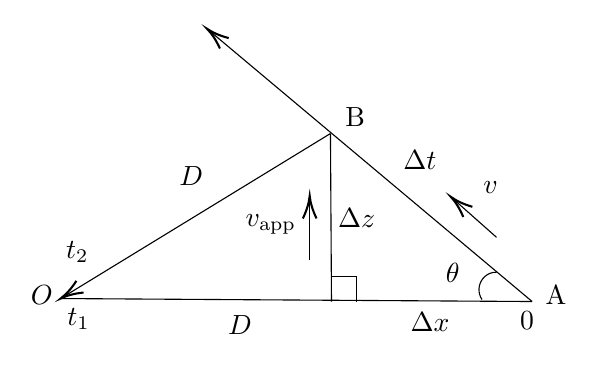
\begin{tikzpicture}[x=0.75pt,y=0.75pt,yscale=-1,xscale=1]
          % 用户提供的 TikZ 代码
          \draw    (23.44,138.06) -- (250.61,139.5);
      \draw    (250.61,139.5) -- (95.48,9.34);
      \draw [shift={(93.94,8.06)}, rotate = 40] [color={rgb, 255:red, 0; green, 0; blue, 0 }  ][line width=0.75]    (10.93,-3.29) .. controls (6.95,-1.4) and (3.31,-0.3) .. (0,0) .. controls (3.31,0.3) and (6.95,1.4) .. (10.93,3.29);
      \draw    (153.44,58.56) -- (25.15,137.01);
      \draw [shift={(23.44,138.06)}, rotate = 328.55] [color={rgb, 255:red, 0; green, 0; blue, 0 }  ][line width=0.75]    (10.93,-3.29) .. controls (6.95,-1.4) and (3.31,-0.3) .. (0,0) .. controls (3.31,0.3) and (6.95,1.4) .. (10.93,3.29);
      \draw  [draw opacity=0] (226.46,138.54) .. controls (225.46,137.07) and (224.91,135.26) .. (225.01,133.33) .. controls (225.25,128.78) and (229,125.26) .. (233.44,125.38) -- (233.2,133.76) -- cycle ; \draw   (226.46,138.54) .. controls (225.46,137.07) and (224.91,135.26) .. (225.01,133.33) .. controls (225.25,128.78) and (229,125.26) .. (233.44,125.38);
      \draw    (153.44,58.56) -- (153.94,139.56);
      \draw   (153.94,127.61) -- (165.83,127.61) -- (165.83,139.56);
      \draw    (233.44,108.56) -- (212.94,90.38);
      \draw [shift={(211.44,89.06)}, rotate = 41.55] [color={rgb, 255:red, 0; green, 0; blue, 0 }  ][line width=0.75]    (10.93,-3.29) .. controls (6.95,-1.4) and (3.31,-0.3) .. (0,0) .. controls (3.31,0.3) and (6.95,1.4) .. (10.93,3.29);
      \draw    (143.44,119.56) -- (143.44,90.56);
      \draw [shift={(143.44,88.56)}, rotate = 90] [color={rgb, 255:red, 0; green, 0; blue, 0 }  ][line width=0.75]    (10.93,-3.29) .. controls (6.95,-1.4) and (3.31,-0.3) .. (0,0) .. controls (3.31,0.3) and (6.95,1.4) .. (10.93,3.29);
      \draw (207.83,119.9) node [anchor=north west][inner sep=0.75pt]    {$\theta $};
      \draw (79.33,73.4) node [anchor=north west][inner sep=0.75pt]    {$D$};
      \draw (102.83,144.9) node [anchor=north west][inner sep=0.75pt]    {$D$};
      \draw (155.83,93.4) node [anchor=north west][inner sep=0.75pt]    {$\Delta z$};
      \draw (190.83,143.4) node [anchor=north west][inner sep=0.75pt]    {$\Delta x$};
      \draw (225.83,80.4) node [anchor=north west][inner sep=0.75pt]    {$v$};
      \draw (7.83,130.5) node [anchor=north west][inner sep=0.75pt]   [align=left] {$O$};
      \draw (255.83,130.5) node [anchor=north west][inner sep=0.75pt]   [align=left] {A};
      \draw (159.33,45) node [anchor=north west][inner sep=0.75pt]   [align=left] {B};
      \draw (111.33,96.4) node [anchor=north west][inner sep=0.75pt]    {$v_{\text{app}}$};
      \draw (243.61,142.9) node [anchor=north west][inner sep=0.75pt]    {$0$};
      \draw (25.44,141.46) node [anchor=north west][inner sep=0.75pt]    {$t_{1}$};
      \draw (24.83,109.4) node [anchor=north west][inner sep=0.75pt]    {$t_{2}$};
      \draw (187.33,65.4) node [anchor=north west][inner sep=0.75pt]    {$\Delta t$};
        \end{tikzpicture}
        \caption{relativistic jet}
        \label{fig:jet}
      \end{figure}

      \begin{align}
        &\Delta z = v\Delta t\sin\theta\label{eq:Deltaz}\\
        &\Delta x = v\Delta t\cos\theta\label{eq:Deltax}\\
        &t_1 = D+\Delta x\label{eq:t1}\\
        &t_2 = D\label{eq:t2}\\
        &\Delta t' = t_1 - t_2\label{eq:nDeltat}
      \end{align}
      Given the apparent velocity definition $v_\text{app}=\frac{\Delta z}{\Delta t'}$ combined with \cref{eq:Deltaz} to \cref{eq:nDeltat}, we can get:
      \begin{equation}
        v_\text{app}=\frac{\Delta z}{\Delta t'}=\frac{v\sin\theta}{1-v\cos\theta}
      \end{equation}
      thus establishing the apparent superluminal motion relation.

      (b)For a given velocity $v$, differentiation of the apparent velocity expression reveals its maximum value occurs at $\theta=\arccos v$:
      \begin{equation}
        v_\text{app}^\text{max}=\frac{v\sqrt{1-v^2}}{1-v^2}=\frac{v}{\sqrt{1-v^2}}
      \end{equation}
      As $v\to 1$, $v_\text{app}\to\infty$. This apparent superluminal motion arises purely from relativistic projection effects, where $v_\text{app}$ represents a geometrical artifact rather than physical particle velocity. Crucially, the true plasma blob velocity $v$ remains subluminal, and no actual information or energy transfer exceeds light speed, thereby fully preserving relativistic causality.

      (c)Given the apparent velocity $v_\text{app}=10$, we substitute this value into the definitional equation:
      \begin{equation}
        v=\frac{10}{\sin\theta + 10\cos\theta}
      \end{equation}
      With the constraint $v\le 1$, to determine the maximum attainable angle $\theta$, we utilize the trigonometric identity $\cos^2\theta + \sin^2\theta = 1$. Solving the coupled equations yields:
      \begin{equation}
        101\cos^2\theta - 200\cos\theta + 99 = 0
      \end{equation}
      Solving this quadratic equation, we get $\theta = \arccos \qty(\frac{99}{101}) \approx \SI{11.4}{\degree}$
\end{solution}

\begin{note}
    
    This geometrically-induced superluminal phenomenon presents intriguing implications. To quantitatively visualize these effects, we employ Python-generated numerical simulations, producing the series of diagrams from \cref{fig:v06} to \cref{fig:vappv}
    % 2x2 多图排版示例
\begin{figure}[htbp]
    \centering
    % 第一行
    \begin{subfigure}[t]{0.48\textwidth}
      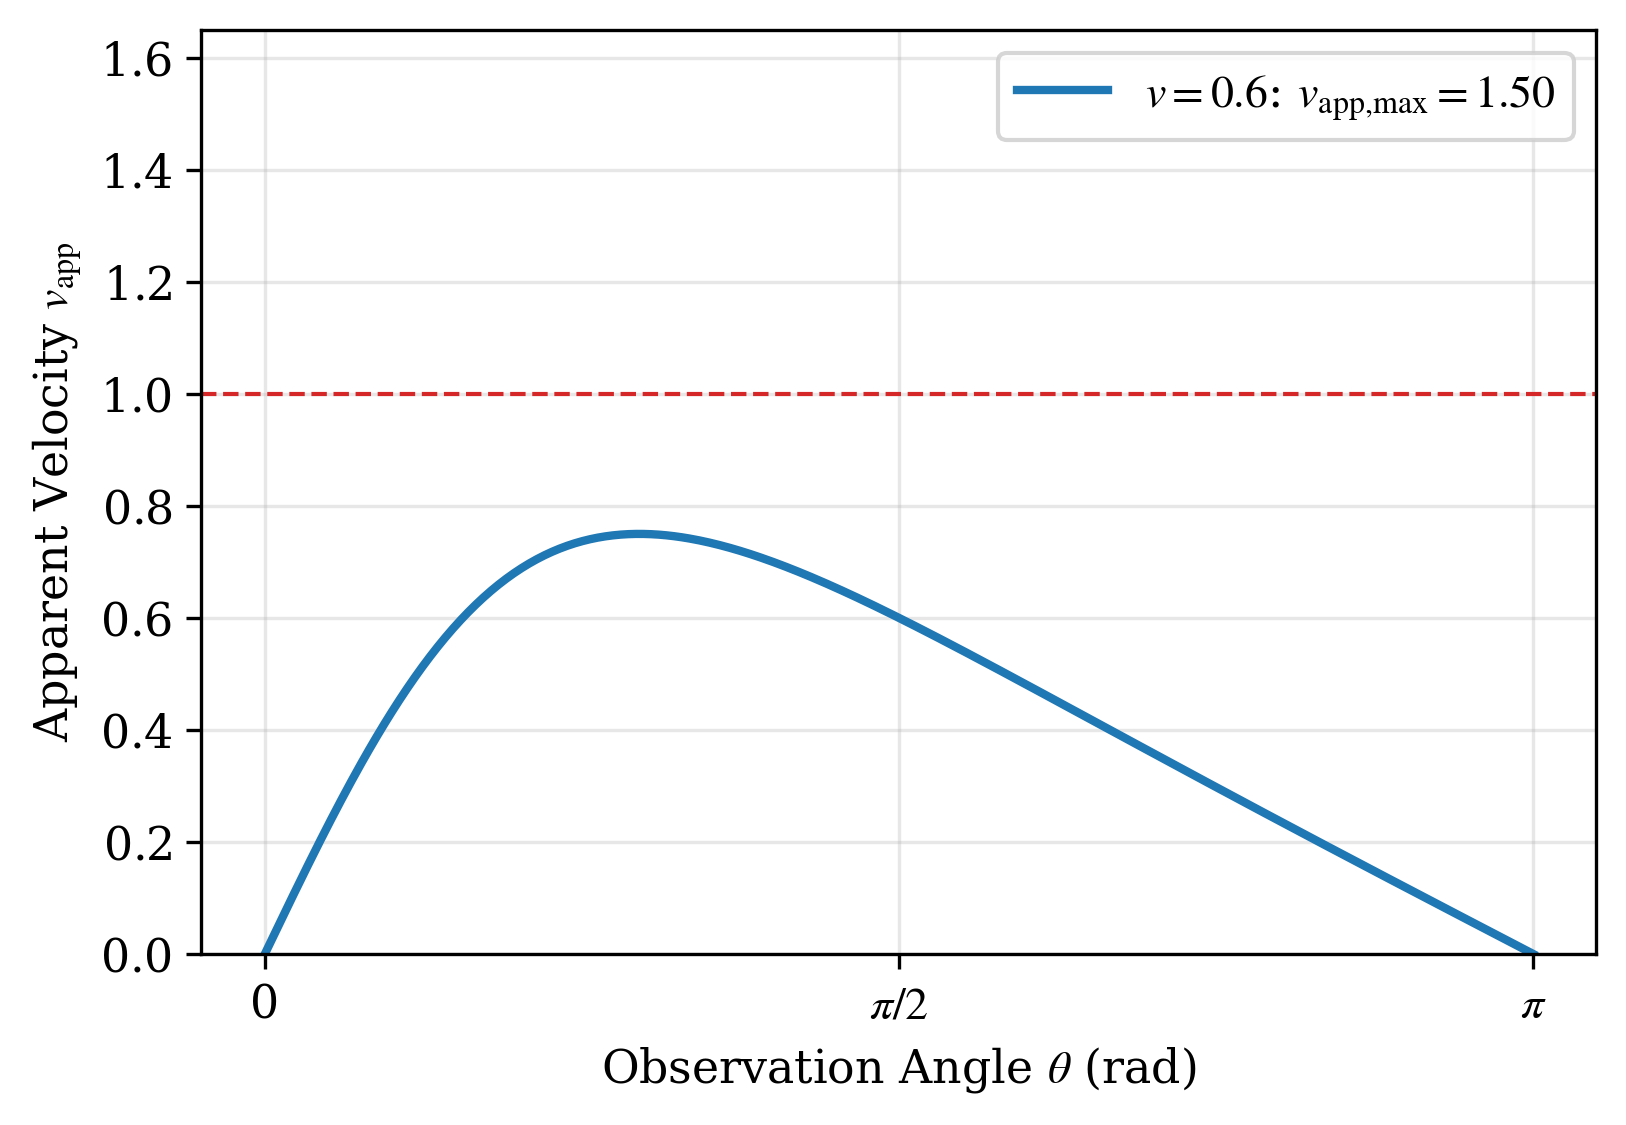
\includegraphics[width=\linewidth]{apparent_velocity_v=0.6.png}
      \caption{$v = 0.6$}
      \label{fig:v06}
    \end{subfigure}
    \hspace*{\fill}  % 自动填充水平间距
    \begin{subfigure}[t]{0.48\textwidth}
      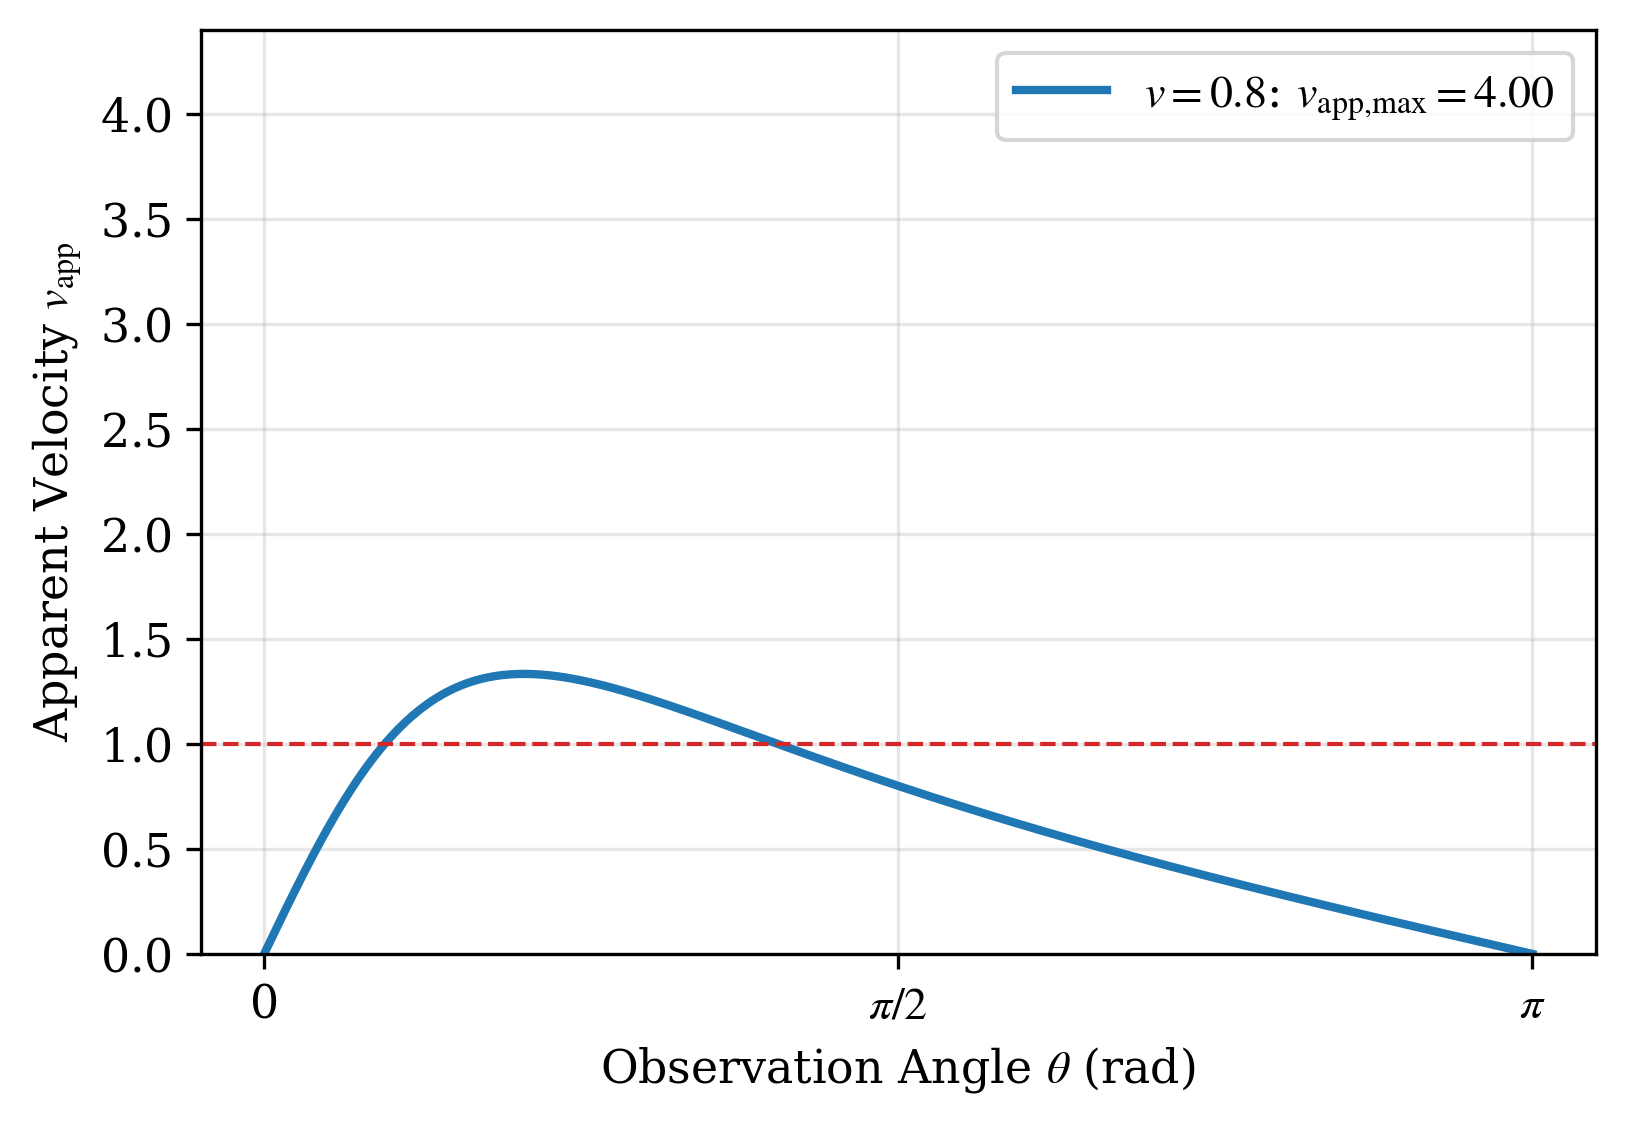
\includegraphics[width=\linewidth]{apparent_velocity_v=0.8.png}
      \caption{$v = 0.8$}
      \label{fig:v08}
    \end{subfigure}
    
    % 第二行
    \vspace{1em}  % 行间距
    \begin{subfigure}[t]{0.48\textwidth}
      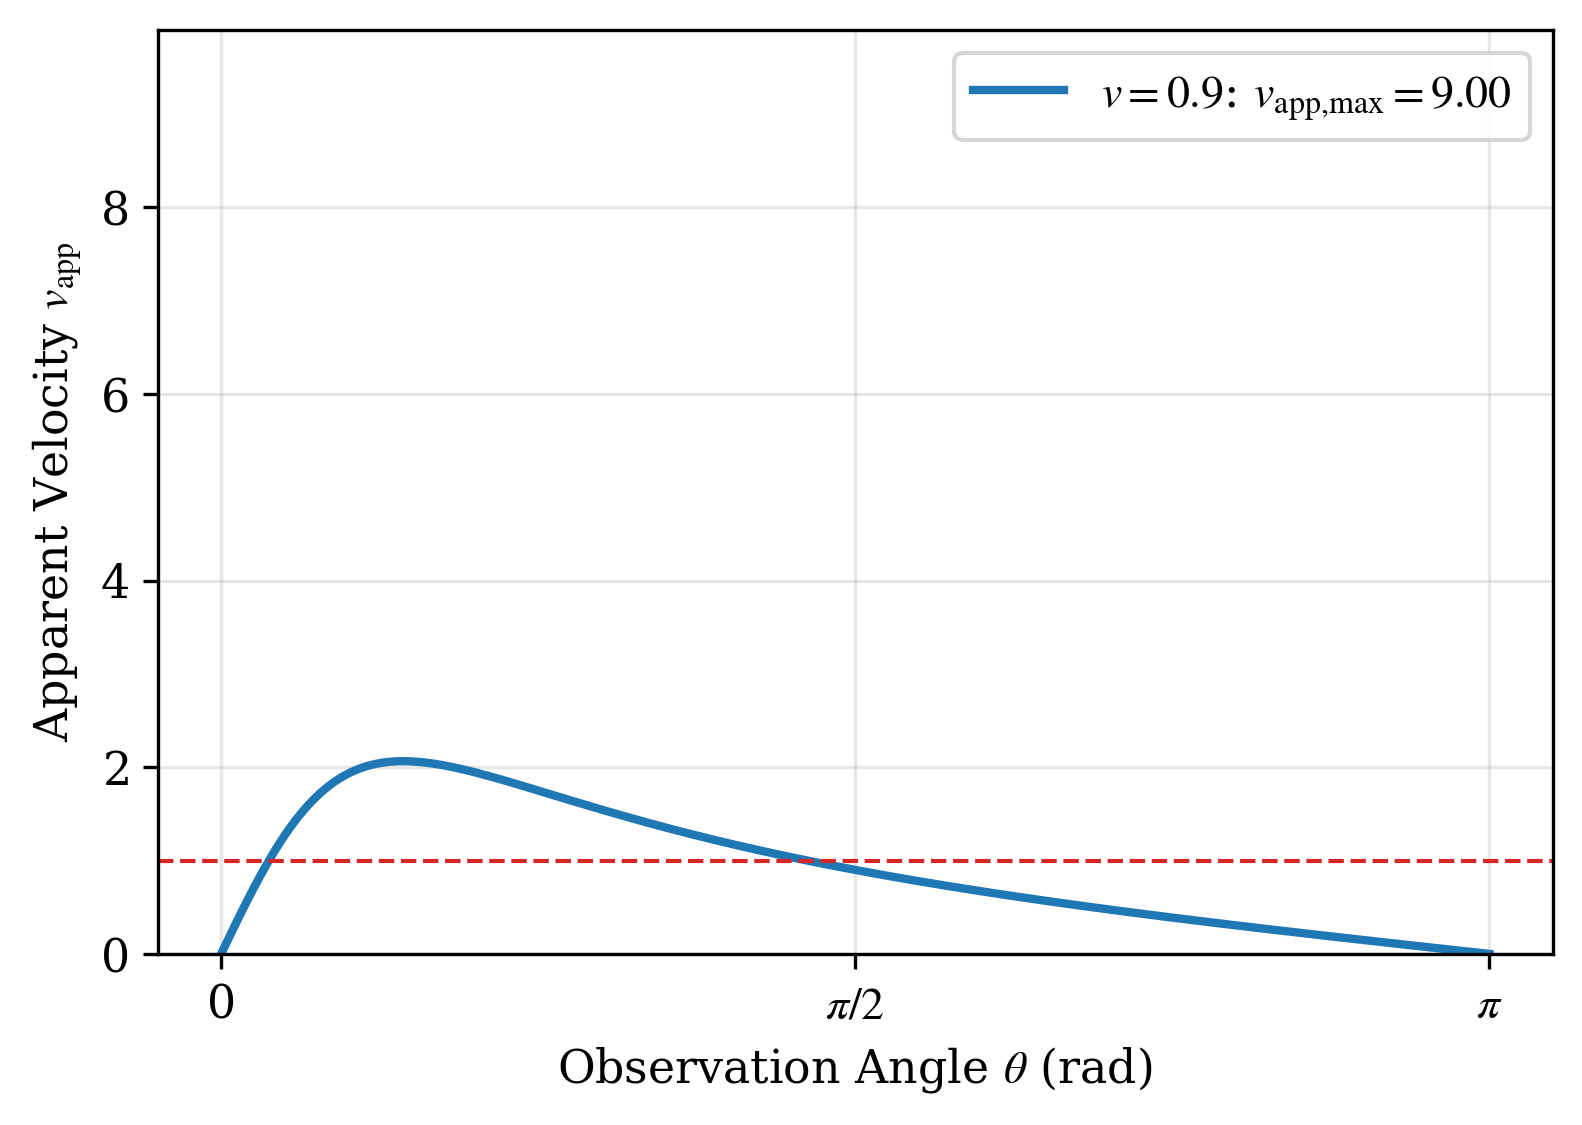
\includegraphics[width=\linewidth]{apparent_velocity_v=0.9.png}
      \caption{$v = 0.9$}
      \label{fig:v09}
    \end{subfigure}
    \hspace*{\fill}
    \begin{subfigure}[t]{0.48\textwidth}
      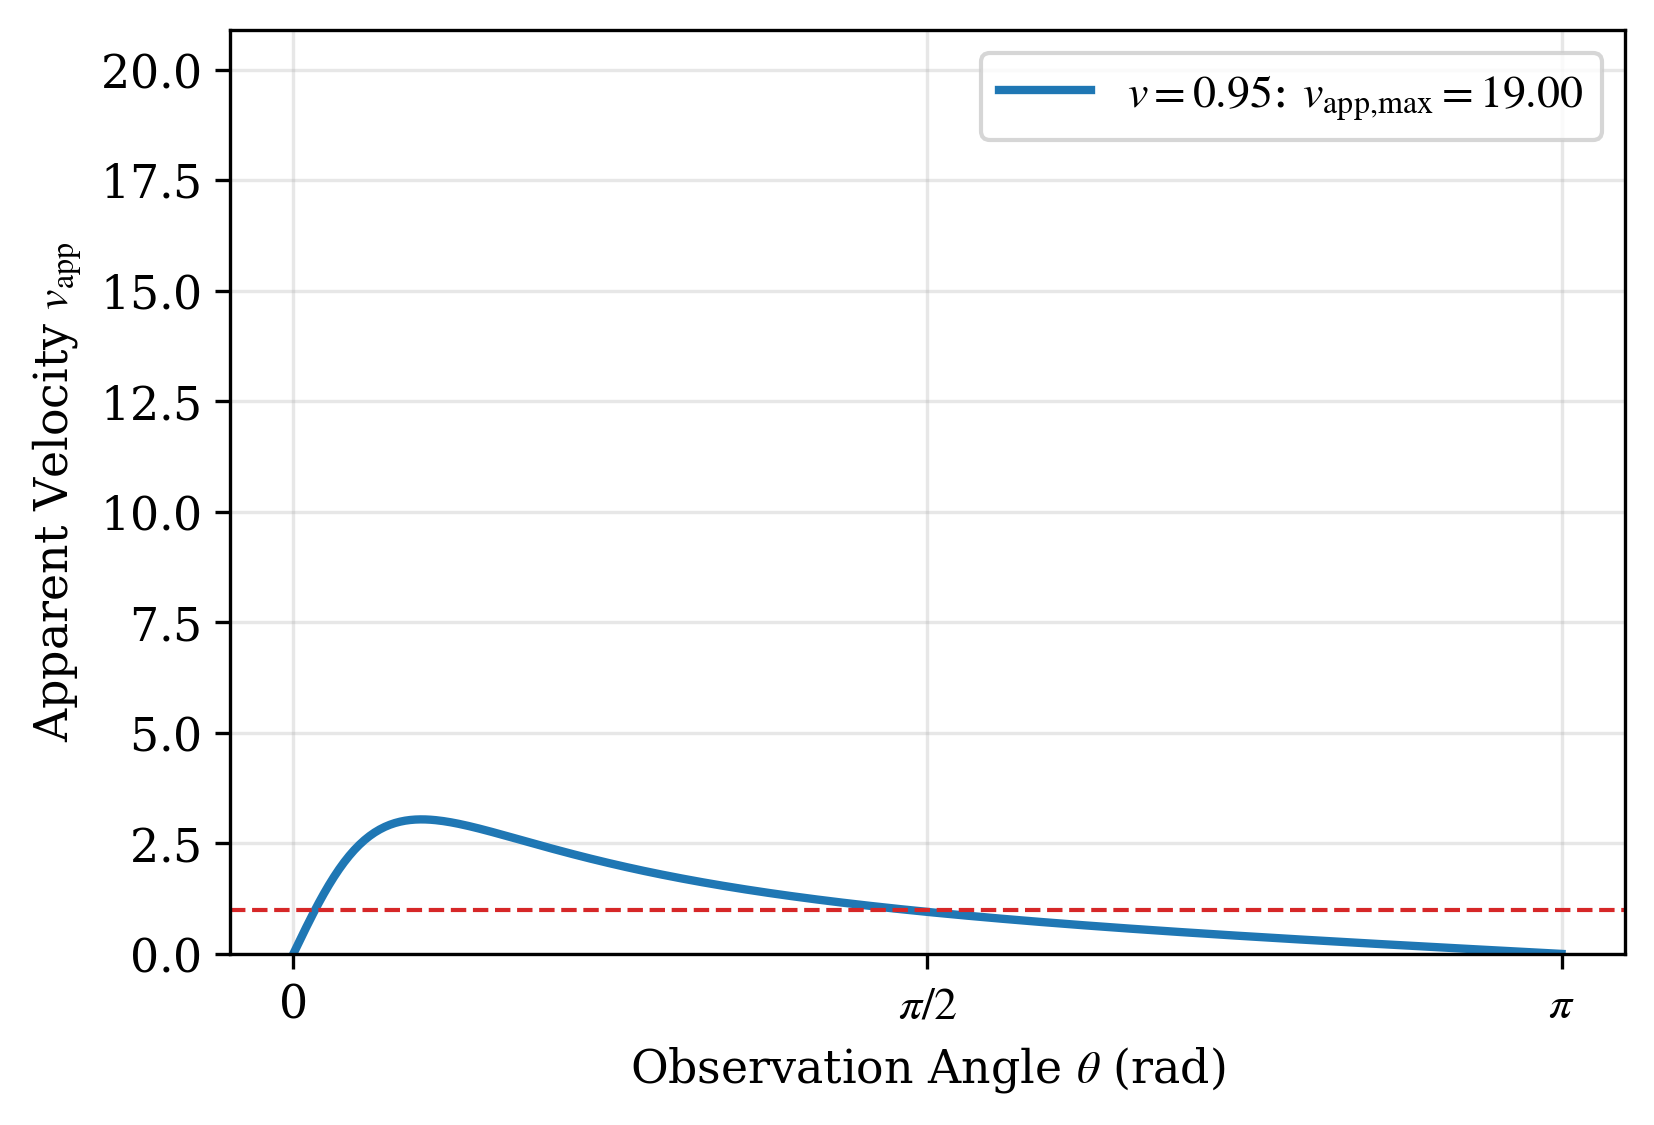
\includegraphics[width=\linewidth]{apparent_velocity_v=0.95.png}
      \caption{$v = 0.95$}
      \label{fig:v095}
    \end{subfigure}
    
    \caption{$v_{\text{app}}$ v.s. $\theta$ for different $v$ in (a)-(d)}
    \label{fig:velocity_grid}
  \end{figure}

  Critical observations from the diagrams include:
  \begin{enumerate}
    \item \textbf{Subluminal Constraint Regime}: At specific fixed velocities $v$, the apparent velocity $v_\text{app}$ remains strictly subluminal regardless of observation angle $\theta$ (exemplified in \cref{fig:v06}).
    \item \textbf{Threshold Condition}: Through rigorous analysis, we establish that superluminal apparent motion occurs if and only if $v\ge\frac{1}{\sqrt{2}}\approx 0.714$
  \end{enumerate}
  \begin{figure}
    \centering
    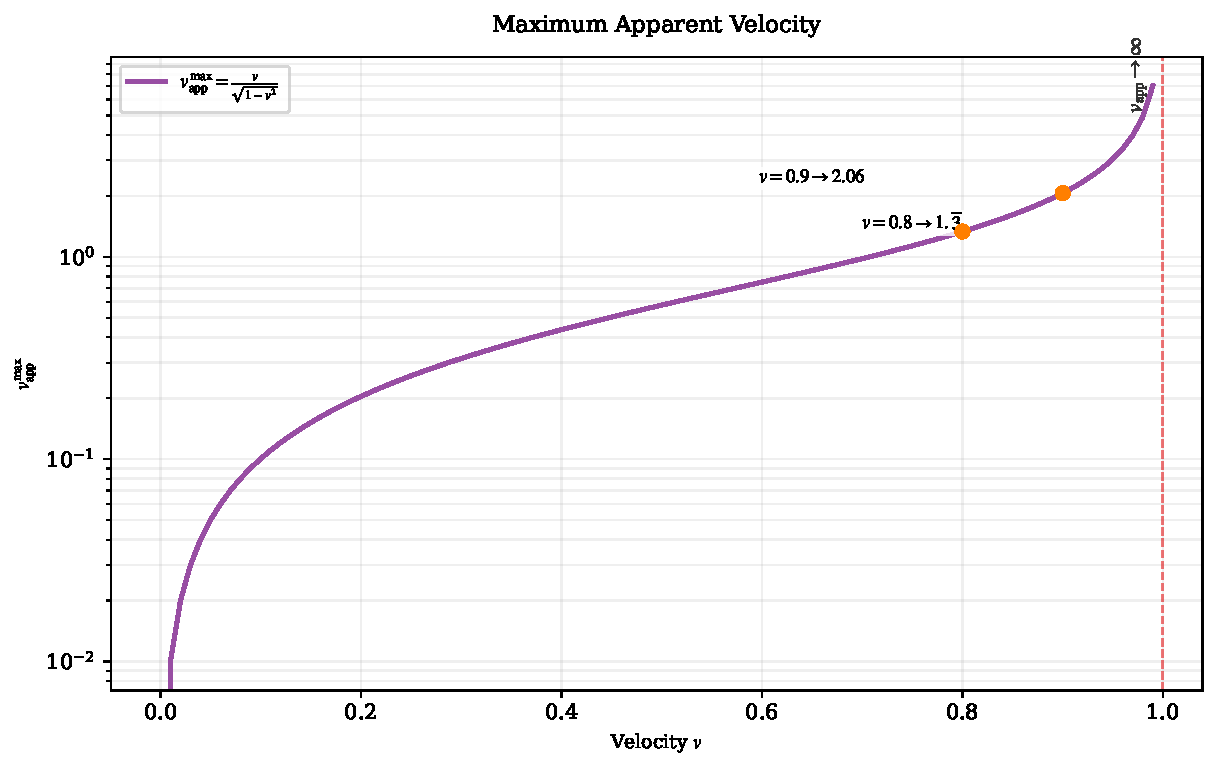
\includegraphics[width=.75\textwidth]{max_apparent_velocity.pdf}
    \caption{$v_\text{app, max}$ v.s. v}
    \label{fig:vappv}
  \end{figure}
\end{note}

\begin{problem}
    GZK cutoff in the cosmic ray spectrum

    (a)Calculate the threshold energy of a nucleon $N$ for it to undergo the reaction $\gamma + N \to N + \pi^0$, where $\gamma$ represents a microwave background photon of energy $kT$ with $T=2.73K$. Assume the collision is head-on and take the nucleon and pion masses to be \SI{938}{MeV} and \SI{135}{MeV}, respectively.

    (b)Explain why one might expect to observe very few cosmic rays of energy above $\sim\SI{e11}{GeV}$.

    (c)This expectation is called the Griesen-Zatsepin-Kuzmin (GZK) cutoff. Modern observations show no sharp cutoff; there may even be evidence for an \textit{upturn} in cosmic ray flux at these energies. Can you suggest a mechanism by which the GZK cutoff can be avoided?
\end{problem}

\begin{solution}
    (a)To determine the nuclear reaction energy threshold, we analyze the critical kinematic condition where the total system energy precisely equals the combined rest mass of the reaction products during a head-on collision. Applying energy-momentum conservation laws:
    \begin{equation*}
        E=m_\text{final}
    \end{equation*}

    Substituting the relativistic energy-momentum relation $E^2_N = p^2_N + m^2_N$:
    \begin{equation}
        \begin{split}
            &(E_N+E_\gamma)^2-(p_N-p_\gamma)^2=(m_N+m_\pi)^2\\
            &\Rightarrow 2E_\gamma(E_N+p_N)=2m_Nm_\pi+m_\pi\\
        \end{split}
    \end{equation}
    Under the high-energy approximation $p_N\gg m_N$:
    \begin{equation}
        \begin{split}
            E_N&=\frac{m_Nm_\pi}{2E_\gamma}\approx\frac{938\times135\times1.60\times10^{-19}}{2\times2.73\times 1.38\times10^{-23}\times10^{-6}}\text{MeV}\\
            &\approx\SI{2.7e14}{MeV}
        \end{split}
    \end{equation}

    (b)The pronounced attenuation of ultra-high-energy cosmic ray flux arises due to the catastrophic energy loss through photopion production processes $\gamma + N \to N + \pi^0$ where cosmic rays interact with cosmic microwave background (CMB) photons. This mechanism, known as the Greisen-Zatsepin-Kuzmin (GZK) cutoff, effectively suppresses particle fluxes beyond the critical energy threshold $E_\text{GZK} \approx \SI{5e19}{eV}$, resulting in the extreme scarcity of observed particles exceeding this energy limit. 
    
    (c)The GZK cutoff may be circumvented under two scenarios:
    \begin{enumerate}
        \item \textbf{Proximity to cosmic ray sources}, where insufficient energy is lost to microwave background photons.
        \item \textbf{Heavy nuclear composition} (e.g., iron nuclei), which possess higher photodisintegration threshold energies.
    \end{enumerate}
\end{solution}

\end{document}